


\documentclass{beamer}
\usepackage{HECbeamer}
% \usepackage{pgfpages}
% \pgfpagesuselayout{4 on 1}[letterpaper, landscape, border shrink=5mm]
\title[\color{white}{MATH 60604A \S~4h - Logistic model for proportions}]{\texorpdfstring{MATH 60604A \\Statistical modelling \\ \S~4h - Logistic model for proportions}{MATH 60604A \\Statistical modelling \\ \S~4h - Logistic model for proportions}}
\author{}
\institute{HEC Montréal\\
Department of Decision Sciences}
\date{} 

\begin{document}
\frame{\titlepage}

\begin{frame}
 \frametitle{Logistic model for proportions}
 
 \bi \item Sometimes, we don't have access to individual records, but rather to aggregated counts such as the number of successes (out of $m$ trials).
 \item We may use a binomial model instead by simply specifying the total number of trials associated to each number of successes.
 \item The parameter interpretation remains the same.
 \ei 
 We consider the pass rate for all 346 Great-Britain driving license practical testing sites; \href{https://www.gov.uk/government/statistical-data-sets/driving-test-statistics-drt}{the data are from 2018}.

\bi 
\item $761\ 750$ people succeeded in their exam out of $1\ 663\ 897$ attempts.
\item \href{https://www.theguardian.com/world/2019/aug/23/an-easy-ride-scottish-village-fuels-debate-driving-test-pass-rates}{A news article from \textit{The Guardian} hinted that exam takers in rural areas got an easy ride.} Since we do not have a classification of urban/rural centers, we use the number of tests conducted as proxy.
\item Other covariates are \texttt{sex} and the \texttt{region} for England; all of Scotland and Wales are pooled.
\ei
 \end{frame}
 \begin{frame}
 \frametitle{Binomial model for driving license pass rate in Great-Britain}
 \begin{center}
  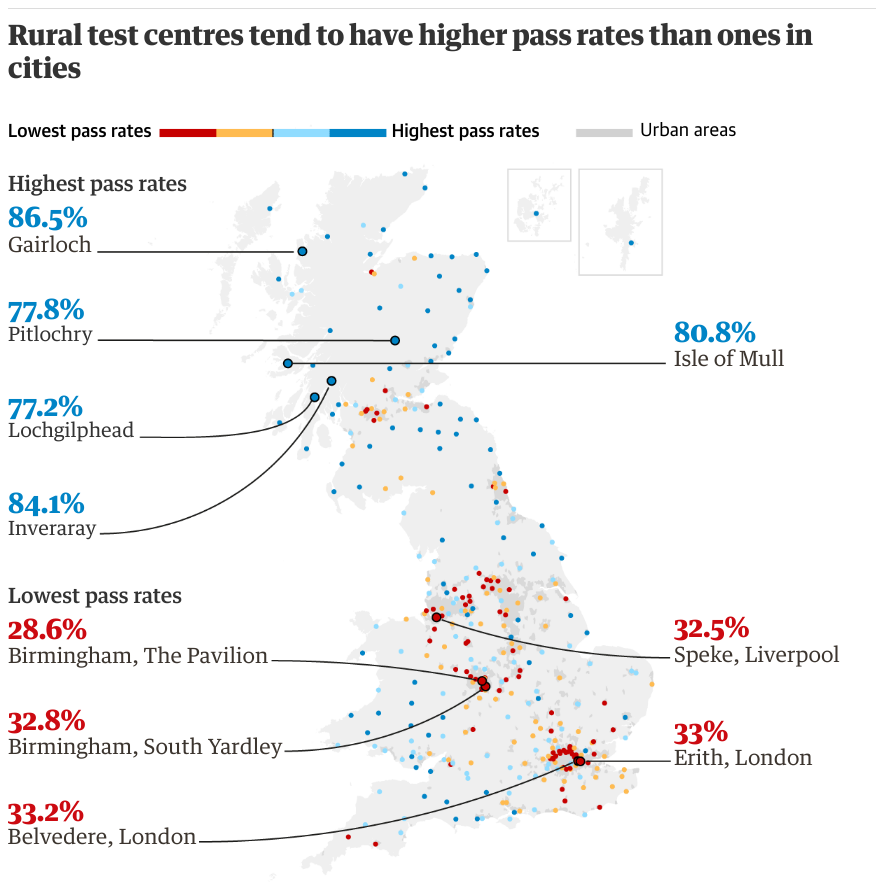
\includegraphics[width = 0.6\linewidth]{img/c4/01-intro-Guardian_UK_driving2.png}
 \end{center}
 {\footnotesize 
Source: \href{https://www.theguardian.com/world/2019/aug/23/an-easy-ride-scottish-village-fuels-debate-driving-test-pass-rates}{The Guardian}.}
\end{frame}
\begin{frame}[fragile]

\begin{tcolorbox}[colback=white, colframe=hecblue, title=SAS code to fit a logistic regression for binomial data]
\begin{verbatim}
data gbdriving;
set statmod.gbdriving;
if(total < 500) then size="small";
else if (total < 1000) then size="medium";
else size = "large";
run;

proc logistic data=gbdriving;
class sex(ref="women") region(ref="London") 
    size / param=glm;
model pass/total = sex region size / 
    plrl plcl expb;
run;
\end{verbatim}
\end{tcolorbox}
\end{frame}
\begin{frame}
 \frametitle{Size of center per region}
 \begin{center}
  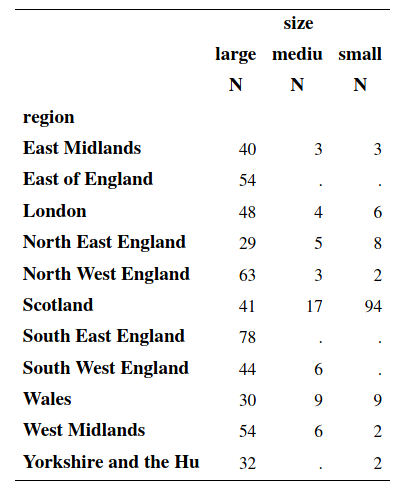
\includegraphics[width = 0.4\linewidth]{img/c4/slides8-e23}
 \end{center}
{ \small Scotland boasts the largest number of small centers (fewer than 500 exams per year).


}
\end{frame}

\begin{frame}
 \frametitle{Model specification for Great-Britain driving licenses}
 \begin{center}
 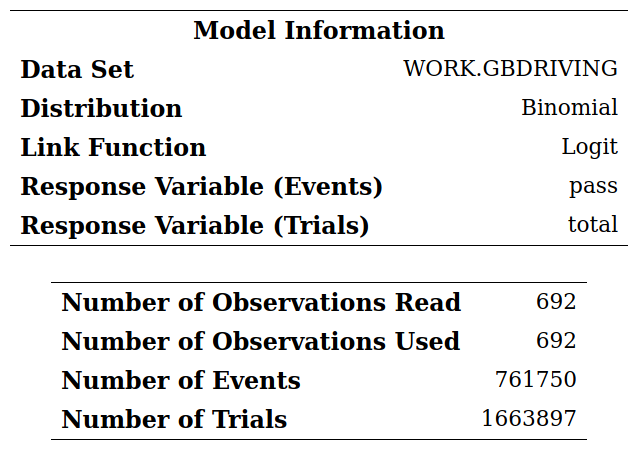
\includegraphics[width = 0.45\linewidth]{img/c4/slides8-e19}
  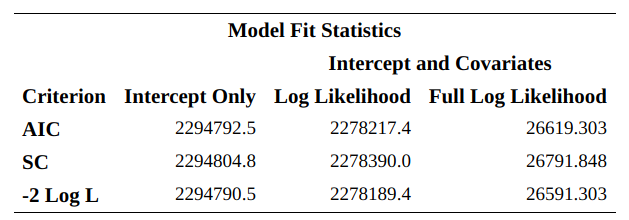
\includegraphics[width = 0.6\linewidth]{img/c4/slides8-e20}
  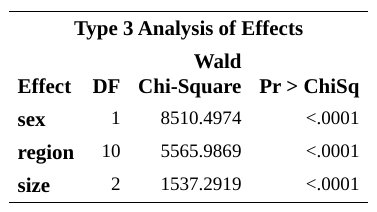
\includegraphics[width = 0.39\linewidth]{img/c4/slides8-e21}
 \end{center}

\end{frame}

\begin{frame}
 \frametitle{Odds estimates for Great-Britain driving licenses data}
 \begin{center}
 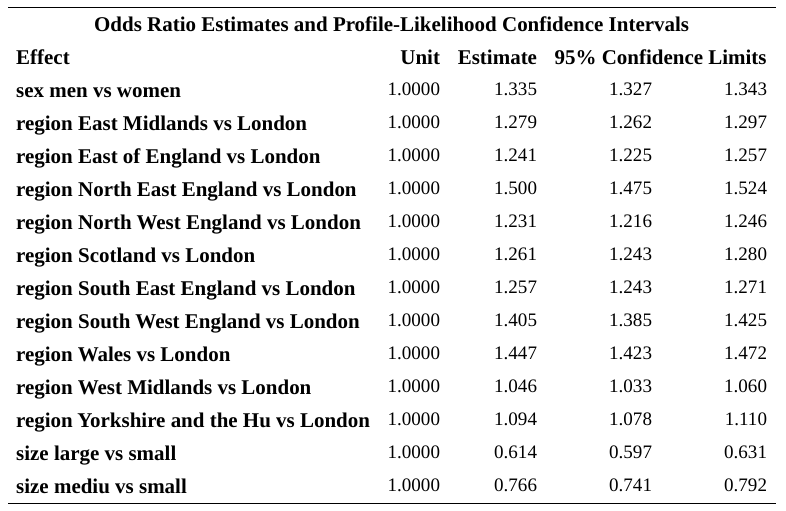
\includegraphics[width = 0.9\linewidth]{img/c4/slides8-e22}
 \end{center}
\end{frame}

\begin{frame}
 \frametitle{Parameter interpretation for Great-Britain driving license}
 All other things being constant,
 \bi \item The odds of men are $33\%$ higher than women of obtaining a driver license;
 \item Greater London is the region with the lowest success rate after accounting for the site volume; the odds of success are $50\%$ higher in North East England and $44.7\%$ higher in Wales, etc.
  \item The odds of success are $63\%$ higher in small center than in large centers ($1/0.614$).
  \item All parameters are statistically significant.
 \ei 
\end{frame}


\begin{frame}
 \frametitle{Remark on models for Bernoulli/binomial data}
 \bi \item While the deviance and Pearson $X^2$ statistics are reported for logistic binomial model, their distribution depends on the unknown parameter vector $\bs{\beta}$.
 \item As such, the deviance is approximately $\chi^2_{n-p-1}$ only when the number of trials $m$ is in the several thousands.
 \item Comparisons of deviance, which amount to likelihood ratio tests, are however valid.
  \ei
\end{frame}

\begin{frame}
 \frametitle{Revisiting the US road casualties example}
 We can fit a binomial model for the \texttt{crash} where the ``event'' is death.
 
 \begin{center}
  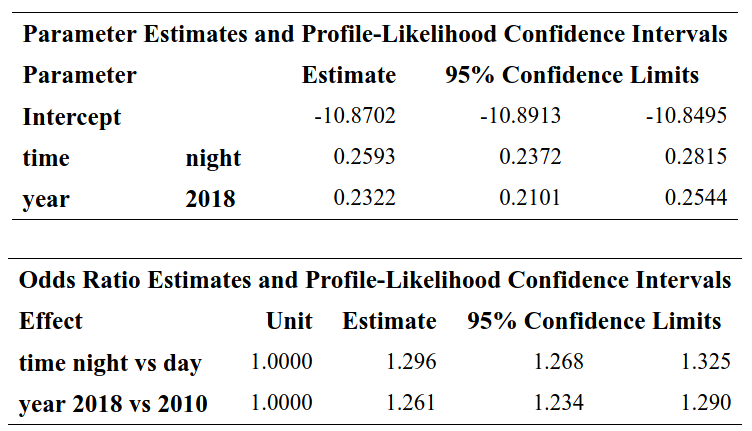
\includegraphics[width = 0.7\linewidth]{img/c4/slides8-e24}
 \end{center}
 {\small
\bi \item The estimated rate of death dying on the road during the day in 2010 is
$\hat{\pi}=\exp(\hat{\beta}_0)/\{1+\exp(\hat{\beta}_0)\} = 0.000019016$, so a death rate of $1.9$ per $100 000$ inhabitants. This estimate is slightly higher than the one from the negative binomial model.
\item The odds of dying during nighttime (relative to daytime) increase by $29.6\%$, whereas the odds for 2018 (relative to 2010) increase by $26.1\%$.
\ei
}
\end{frame}

\end{document}
